% path for images
\graphicspath{{assets/qlearnkit/}}

\section{Qlearnkit}


\begin{frame}{What is Qlearnkit ?}
    \begin{itemize}
        \item a Python library for \alert{Quantum Machine Learning}, built on top of \alert{Qiskit} and (optionally) \alert{Pennylane}
        \item developed at EURECOM for \alert{MALIS} and \alert{QUANTIS}
        \item implements some famous Machine Learning and Deep Learning algorithms and models
        \item open-source and available on Github
        \item installable from PyPi or provided in a Docker container 
        \vspace{0.5cm}
        
        \begin{figure}
            \centering
            \begin{minipage}[c]{0.3\textwidth}
    			
\includegraphics[width=0.4\linewidth]{gh_logo}
    		\end{minipage}
    		\begin{minipage}[c]{0.3\textwidth}
    			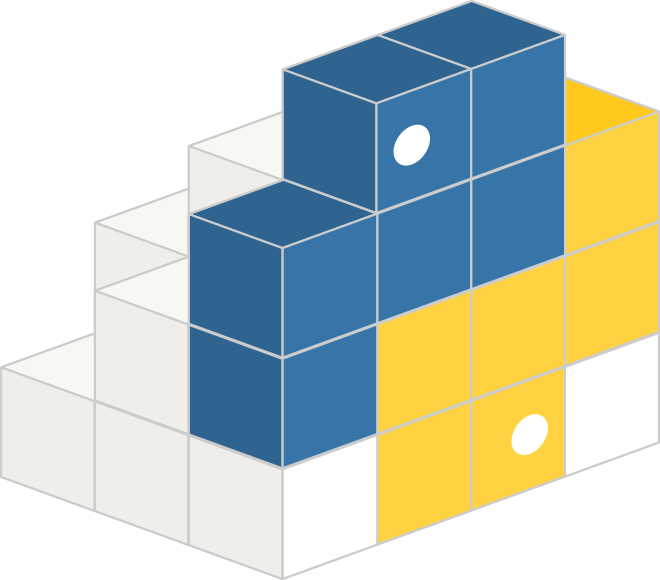
\includegraphics[width=0.4\linewidth]{pypilogo}
    		\end{minipage}
            \begin{minipage}[c]{0.3\textwidth}
			    
\includegraphics[width=0.6\linewidth]{docker-logo}
    		\end{minipage}
        \end{figure}
		
    \end{itemize}
\end{frame}


%%%%%%%%%%%%% QSVM
\subsection{Quantum Support Vector Machines}


\begin{frame}{QSVM - Basic idea}
    Many implementations are possible. The general structure is common:
    \begin{enumerate}
        \item Encode samples in quantum format
        \item Compute a kernel matrix of distances using quantum circuits
        \item Use matrix to solve SVM problem and obtain a solution
    \end{enumerate}
    Steps 2 and 3 can benefit from a quantum speedup. A fully quantum solution has $O(\log mn)$ time complexity 
    
    ($n$: number of features, $m$: number of samples)
\end{frame}

\begin{frame}{An implementation}
    \begin{enumerate}
        \item Encode samples in quantum format
        
        $$ \mathcal{U}_{\Phi(\mathbf{x})}=\prod_d U_{\Phi(\mathbf{x})}H^{\otimes n},\ U_{\Phi(\mathbf{x})}=\exp\left(i\sum_{S\subseteq[n]}\phi_S(\mathbf{x})\prod_{k\in S} P_i\right), $$
        
        Equivalent to mapping in a higher dimensional space.
        \vspace{0.5mm}
        \item Compute a kernel matrix of distances using quantum circuits
        $$K_{ij} = \langle f(\vec{x}_i), f(\vec{x}_j) \rangle = \left| \langle \phi^\dagger(\vec{x}_j)| \phi(\vec{x}_i) \rangle \right|^{2} = 
        |\langle 0^n |\mathcal{U}_{\Phi(\mathbf{x_i})}^{\dagger}\mathcal{U}_{\Phi(\mathbf{x_j})}| 0^n \rangle |^2
        $$
        %Sources: https://arxiv.org/pdf/1804.11326.pdf, https://github.com/Qiskit/qiskit-machine-learning/blob/stable/0.3/docs/tutorials/03_quantum_kernel.ipynb
        Equivalent to computing a scalar product.
    \end{enumerate}
    
    ($n$: number of features, $m$: number of samples)
\end{frame}

\begin{frame}{An implementation}
    \begin{enumerate}
      \setcounter{enumi}{2}
        \item Use this matrix to solve SVM problem and obtain a solution
        LS-SVM Formulation:
            \begin{align*}
            \begin{bmatrix}
            0 & 1^T_N \\
            1_N & K+\gamma^{-1}I_N 
            \end{bmatrix}
            \begin{bmatrix}
            \beta \\
            \alpha
            \end{bmatrix} = 
            \begin{bmatrix}
            0 \\
            Y
            \end{bmatrix}
            \end{align*}
        $\alpha$: SVM parameters
        
        $\beta$: bias term
        
        Predict as
        \begin{align*}
        f(\cdot) = K( \cdot,X) \cdot \alpha + \beta
        \end{align*}
        Note: $K( \cdot,X)$ is done again on a quantum computer
    \end{enumerate}
    
    ($n$: number of features, $m$: number of samples)
\end{frame}



%%%%% QLSTM
\subsection{Quantum Long-Short Term Memory}
\begin{frame}{QLSTM - Basic idea}
	The Quantum Cell is a Variational Quantum Circuit (VQC):
	 
	 \begin{itemize}
	 	\item Encoding Layer for data preparation $\mathcal{U}(X)$ 
	 	\item Variational Layer $\mathcal{V}(\theta)$, with $\theta$ the \alert{learnable} parameters
	 	\item Measurement Layer, to retrieve a \alert{classical} bit string
	 \end{itemize}

	\begin{figure}[h]
		\centering
		\begin{quantikz} 
			& \gate[wires=3][2cm]{\mathcal{U}(\textbf{X})} & \gate[wires=3][2cm]{\mathcal{V}(\boldsymbol\theta)} & \meter{} \\
			& \qw & \qw  & \meter{} \\
			& \qw & \qw  & \meter{} 
		\end{quantikz}
	    \caption{A generic Variational Quantum Circuit with 3 inputs}
	\end{figure}
\end{frame}

%%
\begin{frame}{Architecture}
	%% Architecture without Boxes %%
	 \only<+>{
    \begin{figure}[h]
    	\centering
    	\begin{quantikz}
    		\lstick{$\ket{0}$} & \gate{H} & \gate{R_y} & \gate{R_z} & \ctrl{1} & \qw      & \targ{}  & \gate{R(\alpha_1, \beta_1, \gamma_2)} & \meter{}\\
    		\lstick{$\ket{0}$} & \gate{H} & \gate{R_y} & \gate{R_z} & \targ{}  & \ctrl{1} & \qw & \gate{R(\alpha_2, \beta_2, \gamma_3)} & \meter{} \\
    		\lstick{$\ket{0}$} & \gate{H} & \gate{R_y} & \gate{R_z} & \qw      & \targ{}  & \ctrl{-2} & \gate{R(\alpha_3, \beta_3, \gamma_3)} & \meter{}
    	\end{quantikz}
    	\caption{Single-layer Quantum LSTM cell}
    \end{figure}
	}

	
	
	%% Architecture with 1 Box %%
		\only<+>{
		\begin{figure}[h]
			\begin{quantikz}
				\lstick{$\ket{0}$} & \gate{H}
				
				\gategroup[ 3, % height
				steps=3, % nodes width
				style={dashed, rounded corners,fill=green!30, inner xsep=2pt},
				background,
				label 
				style={label position=below, color=green!90, anchor=north,yshift=-0.2cm}
				] {{\sc encoding layer}}
				
				& \gate{R_y} & \gate{R_z} & \ctrl{1} 
				
				& \qw      & \targ{}  & \gate{R(\alpha_1, \beta_1, \gamma_2)} & \meter{}                
				\\
				\lstick{$\ket{0}$} & \gate{H} & \gate{R_y} & \gate{R_z} & \targ{}  & \ctrl{1} & \qw & \gate{R(\alpha_2, \beta_2, \gamma_3)} & \meter{} \\
				\lstick{$\ket{0}$} & \gate{H} & \gate{R_y} & \gate{R_z} & \qw      & \targ{}  & \ctrl{-2} & \gate{R(\alpha_3, \beta_3, \gamma_3)} & \meter{}
			\end{quantikz}
			\caption{single-layer Quantum LSTM cell}
		\end{figure}
	}
	
	%% Architecture with 2 Boxes %%
		\only<+>{
		\begin{figure}[h]
			\begin{quantikz}
				\lstick{$\ket{0}$} & \gate{H}
				
				\gategroup[ 3, % height
				steps=3, % nodes width
				style={dashed, rounded corners,fill=green!30, inner xsep=2pt},
				background,
				label 
				style={label position=below, color=green!90, anchor=north,yshift=-0.2cm}
				] {{\sc encoding layer}}
				
				& \gate{R_y} & \gate{R_z} & \ctrl{1} 
				
				\gategroup[ 3, % height
				steps=4, % nodes width
				style={dashed, rounded corners,fill=cyan, inner xsep=2pt},
				background,
				label 
				style={label position=below, color=cyan, anchor=north,yshift=-0.2cm}
				] {{\sc variational layer}}
				
				& \qw      & \targ{}  & \gate{R(\alpha_1, \beta_1, \gamma_2)} & \meter{}                
				\\
				\lstick{$\ket{0}$} & \gate{H} & \gate{R_y} & \gate{R_z} & \targ{}  & \ctrl{1} & \qw & \gate{R(\alpha_2, \beta_2, \gamma_3)} & \meter{} \\
				\lstick{$\ket{0}$} & \gate{H} & \gate{R_y} & \gate{R_z} & \qw      & \targ{}  & \ctrl{-2} & \gate{R(\alpha_3, \beta_3, \gamma_3)} & \meter{}
			\end{quantikz}
			\caption{single-layer Quantum LSTM cell}
		\end{figure}
	}
	
	
	
	%% Architecture with 3 Boxes %%
	\only<+>{
		\begin{figure}[h]
		\begin{quantikz}
			\lstick{$\ket{0}$} & \gate{H}
			
			\gategroup[ 3, % height
			steps=3, % nodes width
			style={dashed, rounded corners,fill=green!30, inner xsep=2pt},
			background,
			label 
			style={label position=below, color=green!90, anchor=north,yshift=-0.2cm}
			] {{\sc encoding layer}}
			
			& \gate{R_y} & \gate{R_z} & \ctrl{1} 
			
			\gategroup[ 3, % height
			steps=4, % nodes width
			style={dashed, rounded corners,fill=cyan, inner xsep=2pt},
			background,
			label 
			style={label position=below, color=cyan, anchor=north,yshift=-0.2cm}
			] {{\sc variational layer}}
			
			& \qw      & \targ{}  & \gate{R(\alpha_1, \beta_1, \gamma_2)} & \meter{}
			\gategroup[ 3, % height
			steps=1, % nodes width
			style={dashed, rounded corners,fill=orange!60, inner xsep=2pt},
			background,
			label 
			style={anchor=north, color=orange, yshift=.2cm, xshift=-1.cm}
			] {{\sc measurement layer}}                   
			\\
			\lstick{$\ket{0}$} & \gate{H} & \gate{R_y} & \gate{R_z} & \targ{}  & \ctrl{1} & \qw & \gate{R(\alpha_2, \beta_2, \gamma_3)} & \meter{} \\
			\lstick{$\ket{0}$} & \gate{H} & \gate{R_y} & \gate{R_z} & \qw      & \targ{}  & \ctrl{-2} & \gate{R(\alpha_3, \beta_3, \gamma_3)} & \meter{}
		\end{quantikz}
		\caption{single-layer Quantum LSTM cell}
	\end{figure}
	}
\end{frame}



%%
\begin{frame}{Encoding Layer - Data preparation}
%	\begin{quantikz}
%		& \gate{H} & \gate{R_y(arctan(x_1))} & \gate{R_z(arctan(x^2_1))} & \qw \\
%  		& \gate{H} & \gate{R_y(arctan(x_2))} & \gate{R_z(arctan(x^2_2))} & \qw \\
%  		& \gate{H} & \gate{R_y(arctan(x_3))} & \gate{R_z(arctan(x^2_3))} & \qw 
%	\end{quantikz}
	The \alert{classical} input vector is encoded into rotation angles to "guide" the single-qubit rotations as follows:
	\begin{itemize}
	\item<2-> 
		apply Hadamard to the initial state $|0\rangle \otimes ... \otimes |0 \rangle$ to transform it into an \alert{unbiased} state
		\begin{align*}
			(H | 0 \rangle)^{\otimes N} &= \frac{1}{\sqrt{2^N}} (|0\rangle \otimes ... \otimes |0\rangle + |1\rangle \otimes ... \otimes |1\rangle) 
				=  \frac{1}{\sqrt{2^N}} \sum^{2^N - 1}_0 |i\rangle
		\end{align*}
	  \item<3->
		generate 2N \alert{rotation} angles from the N-dimensional input vector by taking
		\begin{align*}
			\theta_{i,1} = tan^{-1}(x_i), \ \theta_{i,2} = tan^{-1} (x^2_i)
		\end{align*}
		where $\theta_{i,1}$ and $\theta_{i,2}$ are respectively the rotation angles around the y and z axis.
	\end{itemize}
\end{frame}

%%
\begin{frame}{Variational Layer}
	The encoded classical data (now \alert{quantum state}) will go through an entangling layer of CNOTs and single-qubit rotation gates. \\ The 3 rotatio angles \{$\alpha_i, \beta_i, \gamma_i$\} are not fixed in advance, rather they should be updated after every iteration via iterative optimization based on a \alert{gradient descent method}.
\end{frame}

%%
\begin{frame}{Measurement Layer}
	Write me!
\end{frame}


%%
\begin{frame}{Optimization Procedure}
	Write me!
\end{frame}



	